\chapter{Real-time and distributed implementation}\label{ch:chapter_3}


In the previous chapter there is a lack bout data acquisition and transmission, this 
issues are solved over a distributed computing approach. In this chapter are described the implementation of the developed drivers for OpenBCI over a distributed frame. This feature use a distributed event store and stream-processing platform called \textit{Apache Kafka} for the data transmission through the network, this same network is also used to deploy web servers and synchronize the systems. All this set defines the real-time conditions and describe the operating condition of the BCI system implemented.


%======================================================================
\section{Real-time}

The real-time definition used to describe the purposed system is based on the sampling blocks transmission, the system developed guarantees that all EEG data blocks of duration $P$ will be \textit{available} for the user in a time lower that $P$, no matters the duration of the block. In this case \textit{available} refers to ready to use data in the development environment.

This definition arises from the need to compare different system configurations. Given that the obtained acquisition system is highly configurable about sampling rate, numbers of channels, protocols, and block of data transmitted. Express the latency in percentage terms simplify the comparison of the capabilities when a BCI system is designed and developed.

%======================================================================
\section{Kafka: Open-source distributed event streaming platform}

The core of the distributing system resides in Kafka, this software is fast enough to implement real-time applications and so simple to be based on binary data transmission. The main platform run under Java but there is a wrapper called \footcite{kafka-python}{https://kafka-python.readthedocs.io/en/master/} that able the programming inside python environments.

In addition to all the infrastructure that Kafka brings to the system, when used in the development of a system, this work only will refers to the main features related to read and send stream data: Produsers, consumers and generators scripts.


%----------------------------------------------------------------------
\subsection{Topics}

Kafka protocol is so simple that the identifiers consist of a single string called \textit{topic}, this topic are categories used to organize messages. Internally they are configured by other features like, \textit{replication factor} and \textit{partitions}, our implementation consist only in one server, in order to speed-up the message transmission by avoiding the triggering and the redundant message allocation. The topics needs explicit definition, there can not be created on run-time.

%----------------------------------------------------------------------
\subsection{Producer}

From a coding perspective, the producers consist of scripts that feed the streaming with new data, then Kafka distribute this messages to all nodes connected. Since Kafka only comprise the transmission of binary data, all messages involved are serialized in producers and  de-serialized in consumer using the Python standard library \quot{pickle}.

\begin{python}
from kafka import KafkaProducer
producer = KafkaProducer()

for _ in range(100):
    producer.send('my_topic', b'some_message_bytes')
\end{python}

In order to run this scripts, the Kafka service must be running in background. 

%----------------------------------------------------------------------
\subsection{Consumer}

The scripts that implement a Kafka consumer are based on asynchronous callbacks:

\begin{python}
from kafka import KafkaConsumer

consumer = KafkaConsumer()
consumer.subscribe(['my_topic'])
for msg in consumer:
    print(msg)
\end{python}

%----------------------------------------------------------------------
\subsection{Transformer}

The transformer are a combination of consumers and producers, this kind of scripts consume data from the stream and then stream back with a different topic. The transformers are useful to parallelize process.


%======================================================================
\section{Distributed system implementation}

The distributed implementation is used to isolate the acquisition system, since this is not running under a real-time operating system, the latencies can turn into unstable ranges due other non related computational process running in background. 

Centralized process are also susceptible to high computational demanding processing tasks, if a BCI system is under development the performance could vary in part only due the available resources, compromising the comparability of the evaluated models.

%----------------------------------------------------------------------
\subsection{Remote Python Call}

The \gls*{RPyC} Python module enable the execution through network of wrapped modules, this module require a few configurations to start serving object-proxying to overcome the physical boundaries between processes and computers, so that remote objects can be manipulated as if they were local.

Although the module requires a custom scripting in order to access to object-proxying, with the aim to simplify the implementation of the drivers a transparent configuration have been included in the development. The argument \quot{host} refers and initialize the connection with the remote module running in the pointed server. All methods, commands and responses generated are processed in the same way that local are, them, the user will not notice any difference from use the library with a local or a remote OpenBCI device. 

\begin{python}
from openbci_stream.acquisition import Cyton

openbci = Cyton('serial', host='192.168.1.1', endpoint='/dev/ttyUSB0', capture_stream=True)
openbci.stream(15)  # capture 15 seconds of data
openbci.eeg_time_series # Raw EEG is allocated in this class instance
\end{python}

%======================================================================
\section{Isolated acquisition}\label{chap3:isolated-acquisition}

Once defined the distributed system, a recommended step is move the acquisition into a isolated environment. A dedicated operating system that only executes the daemons and process related to the acquisition as well as the Kafka server. This system also can be configured as a Wi-Fi access point, needed to handle the OpenBCI through the Wi-Fi module. All this tasks can be implemented into a \gls*{SBC} using a operating system based on a minimalist distribution of GNU/Linux.

For the development of this work, a preconfigured environment for Raspberry Pi was developed using \textit{Archlinux ARM}, although \textit{Manjaro ARM Minimal} can also be used, the configuration is described in the \footcite{documentation}{https://openbci-stream.readthedocs.io/en/latest/notebooks/A3-server-based\_acquisition.html} as a simple terminal command over a fresh installation.

This distribution enable the Raspberry Pi as a \textit{plug and play} acquisition server. Every time that the system boot this one will be configured as A \gls{RTP} server and a Wi-Fi access point, the Kafka server will start to running in background, the binary deserializer daemon start listening binary data, and the EEG streamer start to listening  deserialized data, and the RPyC server starts wrapping the drivers.

Although the \gls*{RPyC} module brings access to the EEG data, this protocol is not enough for the high rate transmissions needed for configurations of 1000 \gls*{SPS} and 16 channels. For this reason Kafka is used to distribute data even when there is only one client involved.

%----------------------------------------------------------------------
\section{Electrode impedance measurement}\label{subsec:impedance-measurement}

A low impedance electrode-skin is always recommended because, under low ranges, the effect on the amplifications remains at low levels, even lower than the resolution of \Gls*{ADC}. The \footcite{ADS1299}{https://www.ti.com/product/ADS1299} in the analog-to-digital converter for biopotential measurements is implemented in \textit{OpenBCI}: this microcontroller includes a way to perform the impedance measure using the lead-off current sources. 

This method consists of injecting a small current of $6 nA$ at $31.2 Hz$. The signal acquired is processed to calculate the $V_{RMS}$ voltage and then the impedance $Z$ using Ohm’s law. 

\begin{python}
openbci = Cyton(
    'wifi',
    '192.168.1.113',
    host='192.168.1.1',
    capture_stream=True,
    daisy=False,
)

openbci.command(cons.SAMPLE_RATE_250SPS)
openbci.command(cons.DEFAULT_CHANNELS_SETTINGS)
openbci.leadoff_impedance(
    range(1, 9),
    pchan=cons.TEST_SIGNAL_NOT_APPLIED,
    nchan=cons.TEST_SIGNAL_APPLIED,
)

openbci.stream(7)
data_raw = np.array(openbci.eeg_time_series)
\end{python}

\begin{figure}
\begin{centering}
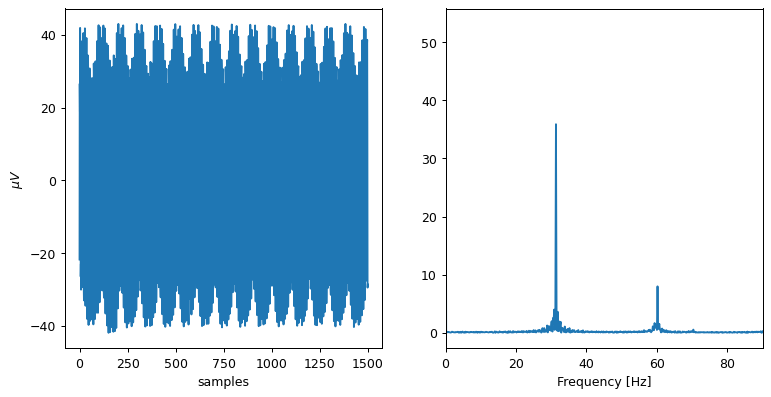
\includegraphics[width=0.8\textwidth]{Cap2/Figures/imedances_signal.png}
\par\end{centering}
\caption{Raw signal for the \textit{lead-off} configuration.}
\label{fig:bci_drivers}
\end{figure}

\begin{python}
band_2737 = GenericButterBand(27, 37, fs=250)
data = band_2737(data_raw)
\end{python}

\begin{figure}
\begin{centering}
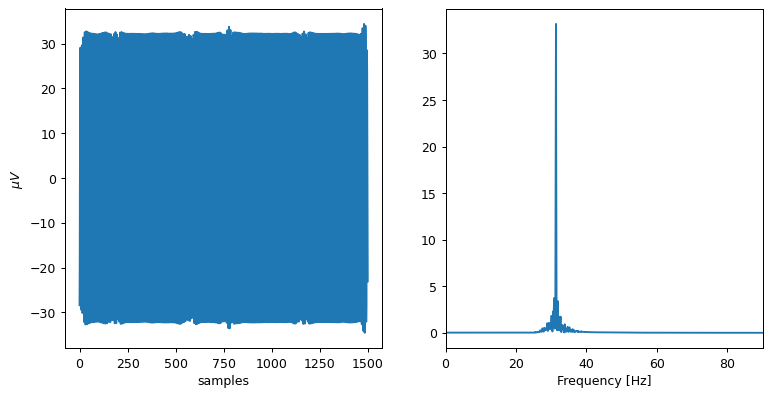
\includegraphics[width=0.8\textwidth]{Cap2/Figures/imedances_signal_filtered.png}
\par\end{centering}
\caption{Filtered signal for the \textit{lead-off} configuration.}
\label{fig:bci_drivers}
\end{figure}

The $V_{RMS}$ can be calculated as the \quot{std()} of the voltage array.

\[
V_{RMS}=\frac{V_{pp}}{2\sqrt{2}}\thickapprox std(V) 
\]

This is how our $I_{RMS}$ can be calculated:

\[
I_{RMS}=\frac{6nA}{\sqrt{2}}
\]


Then the impedance $Z$ is...

\[
Z=\frac{V_{RMS}}{I_{RMS}}
\]

Since the $V_{RMS}$ and the $std(V)$ are by default in $\mu V$, this would be the impedance measured for a vector of data $V$:

\[
Z=\frac{std(V)\cdot10^{-6}\cdot\sqrt{2}}{6\cdot10^{-9}}\:\Omega
\]

The Cyton board has a 2.2K Ohm resistors in series with each electrode, so we must remove this value in way to get the real electrode-to-head impedance.


%----------------------------------------------------------------------
\subsubsection{Real time measurement}
For this experiment we will use the Kafka consumer interface, and the same potentiometer. Keep in mind that this measurement uses one second signal, so, the variance will affect the real measure, in real-life the amplitude not change so drastically.

\begin{python}
from openbci_stream.acquisition import OpenBCIConsumer
from openbci_stream.acquisition.cyton_base import CytonConstants as cons
from openbci_stream.utils.filters import GenericButterBand
import numpy as np
import time

def get_rms(v):
    return np.std(v)

def get_z(v):
    rms = get_rms(v)
    z = (1e-6 * rms * np.sqrt(2) / 6e-9) - 2200
    if z < 0:
        return 0
    return z

Z = []
band_2737 = GenericButterBand(27, 37, fs=250)
with OpenBCIConsumer(
    'wifi',
    '192.168.1.113',
    host='192.168.1.1',
    auto_start=False,
    streaming_package_size=250,
    daisy=False,
) as (stream, openbci):
    # with OpenBCIConsumer(host='192.168.1.1') as stream:

    openbci.command(cons.SAMPLE_RATE_250SPS)
    openbci.command(cons.DEFAULT_CHANNELS_SETTINGS)
    openbci.leadoff_impedance(
        range(1, 9),
        pchan=cons.TEST_SIGNAL_NOT_APPLIED,
        nchan=cons.TEST_SIGNAL_APPLIED,
    )
    time.sleep(1)
    openbci.start_stream()

    for i, message in enumerate(stream):
        if message.topic == 'eeg':
            eeg, aux = message.value['data']
            eeg = band_2737(eeg)
            z = get_z(eeg[0])
            Z.append(z)
            print(f'{z/1000:.2f} kOhm')

        if i >= 15:
            break
\end{python}
\begin{figure}
\begin{centering}
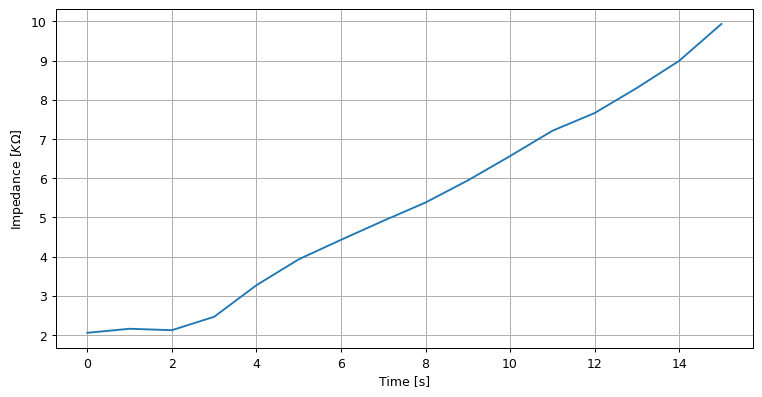
\includegraphics[width=0.8\textwidth]{Cap2/Figures/imedances_signal_pot.png}
\par\end{centering}
\caption{Real-time impedance measurement of a 10 KOhm potentiometer.}
\label{fig:bci_drivers}
\end{figure}

This measure needs a block of data to obtain a stable value. Although the method used to calculate the $V_{RMS}$ is fast, the \quot{std()}, at non-stationary times, such as while the electrode is fixed or manipulated, will affect the impedance measurement, so the calculated value will not be accurate. The measure impedance protocol requires rest periods before interpreting the value calculated.

Some recommendations for improving the impedance measurement can be:
(i) Take shorts signals but enough, 1 second is fine. 
(ii) Remove the first and last segments of the filtered signal.
(iii) Nonstationary signals will produce wrong measurements.
(iv) A single measurement is not enough, is recommended to work with trends instead.

%======================================================================
\section{Latency analysis} 

The latency comprise the time elapsed between the acquisition of raw EEG data from the OpenBCI board and the availability in the development framework. This analysis was performed over a complete distributed system and the following conditions: (i) The OpenBCI acquisition system was isolated in a dedicated Raspberry Pi, (ii) The data was read in a remote computer using the developed drivers, (iii) The block size was fixed in 100 samples, and (iv) The samples per second was fixed in 1000. The system was designed in a way that all times are registered and streamed alongside the main EEG data. This feature able to developers to perform a latency analysis without configure a special mode, this means that use the same conditions of a EEG acquisition session. 


\begin{figure}
\begin{centering}
% \includesvg[width=0.8\textwidth]{Cap4/Figures/transformer.svg}
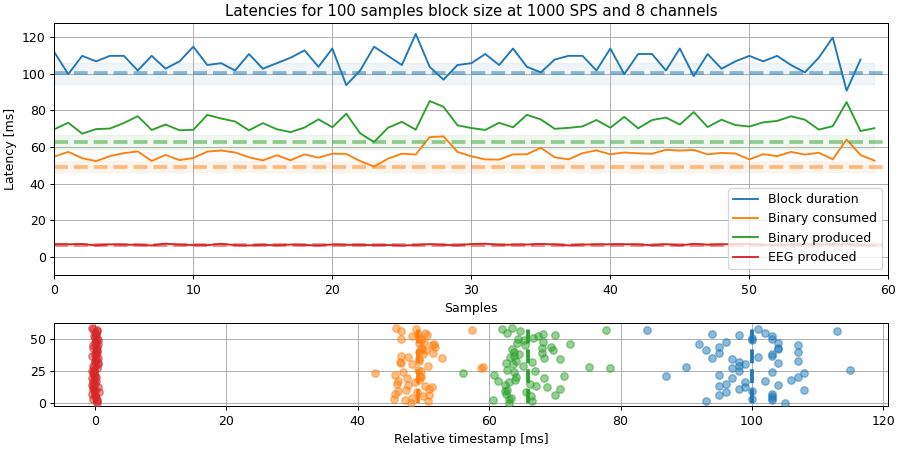
\includegraphics[width=1\textwidth]{Cap3/Figures/100ms1000sps_latencies.png}
\par\end{centering}
\caption[Latencies for 100 samples block size and 1000 SPS.]{Latencies for 100 samples block size and 1000 SPS. The latencies show the elapsed time from reading the packet to the time of packaging. The dashed line mark the minimum latency and the shade is the standard deviation for all segment.}
\label{fig:latencies_100ms}
\end{figure}

In figure \ref{fig:latencies_100ms} are plotted four relative timestamps and compared with the block duration. The \textit{Binary produced} is the time elapsed since the raw data was acquired and streamed through Kafka, \textit{Binary consumed} is the time elapsed since the binary data was consumed, just before to the deserialization, \textit{EEG produced} refers to the duration of the transmission, this is the time since the thee EEG was inserted in the Kafka stream and read in the final consumer.
There is a few facts about this plot that needs to be mentioned, 
The difference between zero and \textit{EEG produced} also includes the clock offset. 
The time bewteen \textit{Binary consumed} and \textit{EEG produced} is the time spent on the deserialization of the raw data.
The time bewteen \textit{Binary produced} and \textit{Block duration} is the time spent on the acquisition of the EEG data, this is the latency acquisition of OpenBCI when its works over the WiFi protocole. 
We can conclude then, that the deserialization process is highly time expensive.

\begin{figure}
\begin{centering}
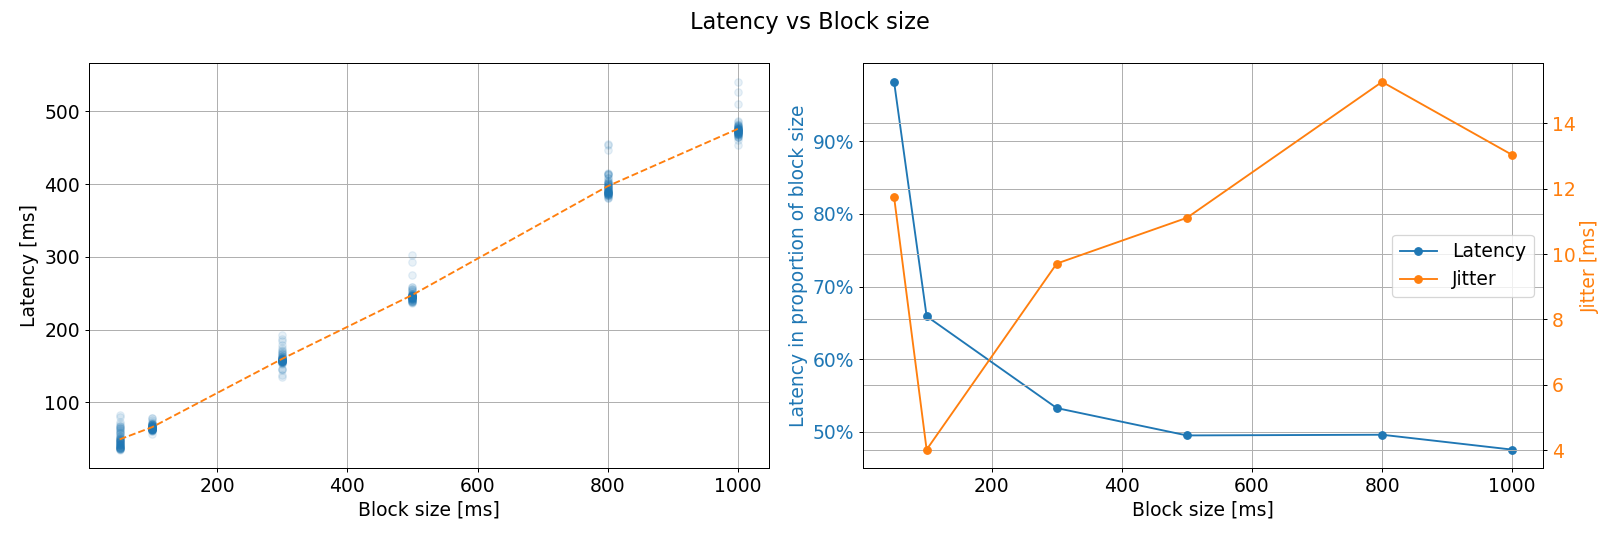
\includegraphics[width=1\textwidth]{Cap3/Figures/block_vs_latency.png}
\par\end{centering}
\caption[Latency vs Block size]{Latency vs Block size. 
In the left is possible to see that the latency is proportional to the block size. 
In the right plot, the latency decrease for small block size but their standard deviation (jitter) increase. 
The preferred configuration was set up in 100 samples block size due the lower jitter.}
\label{fig:latency_vs_block}
\end{figure}

The same process was performed for six different block sizes keeping the same 1000 SPS, the results are showed in Figure \ref{fig:latency_vs_block}, only the \textit{Binary produced} is compared with the \textit{Block size}. For block sizes under the 1000 samples and up to 100 the latency seems to be lineal.
If the data is represented using the percentage as a comparison measure, the latency seems to stabilize in $50 \%$, however the jitter appear to increase with block size. This results suggest that the optimal configuration for the EEG acquisition, using the developed drivers, is around 100 samples block size with only 8 ms of jitter.

% Preview source code for paragraph 13

\begin{table}
\begin{centering}
\begin{tabular}{>{\raggedright}p{3.3cm}cccccc}
\toprule 
\addlinespace[1em]
\textbf{BCI system} & \textbf{Sample rate} & \textbf{Block size} & \textbf{Jitter} & \textbf{Communication} & \textbf{Distributed} & \textbf{Latency}\tabularnewline\addlinespace[1em]
\midrule
\addlinespace[1em]
\textbf{BCI2000 + DT3003 \cite{schalk2004bci2000}} & 160 Hz & 6.35 ms & 0.67 ms & Wired & No & \textbf{51.9 \%}\tabularnewline
\addlinespace[0.5cm]
\textbf{BCI2000 + NI 6024E \cite{schalk2004bci2000}} & 25 kHz & 40 ms & 0.75 ms & Wired & No & \textbf{27.5 \%}\tabularnewline
\addlinespace[0.5cm]
\textbf{BCI2000 + g.USBamp \cite{wilson2010procedure}} & 1200 Hz & 83.3 ms & 5.91 ms & Wired & No & \textbf{14, 30, 48 \%}\tabularnewline
\addlinespace[0.5cm]
\textbf{OpenViBE + TMSi Porti32 \cite{kisakye2013brain}} & 512 Hz & 62.5 ms & 3.07 ms & Optical MUX & No & \textbf{100.4 \%}\tabularnewline
\addlinespace[0.5cm]
\textbf{BCI-Framework} & \textbf{1000 Hz} & \textbf{100 ms} & \textbf{5.7 ms} & \textbf{Wireless} & \textbf{Yes} & \textbf{56 \%}\tabularnewline\addlinespace[1em]
\bottomrule
\addlinespace[0.5cm]
\end{tabular}
\par\end{centering}
\caption{Latencies comparison, the latency has been expressed in terms of percentage of the block size to make the possible the comparison between different systems configurations.\label{table:latencies-comparison}}
\end{table}




Table \ref{table:latencies-comparison} show a comparison between different BCI systems configurations. The wired systems has significantly lower jitter than wireless. For centralized implementations like \textit{BCI2000 + g.USBamp} the latency depends also of the paradigm, then, the same configuration have different latencies responses.






%======================================================================
\section{Sampling analysis} 

The sampling is the process to acquire data at fixed sample rate, the acquisition process must gather the a uniform sampling rate of the signal. It is inevitable to lose data, there are some reasons, like lags in the Wi-Fi connection, in the acquisition board or in the operating system. If it is assumed that the acquisition is homogeneous, then, after a session of EEG all data will be widen to cover the supposed duration of the experiment. This will drive to an incorrect partitioning of trials. OpenBCI includes a set of special features that can be used to detect this anomalies. The first one is to use the sample indexes to detect when a data is not transmitted, and the second consist of to use known test signal. Additional to this ones, the developed drivers include a timestamp annotation for each sample that can be used too.


\begin{figure}
\begin{centering}
% \includesvg[width=0.8\textwidth]{Cap4/Figures/transformer.svg}
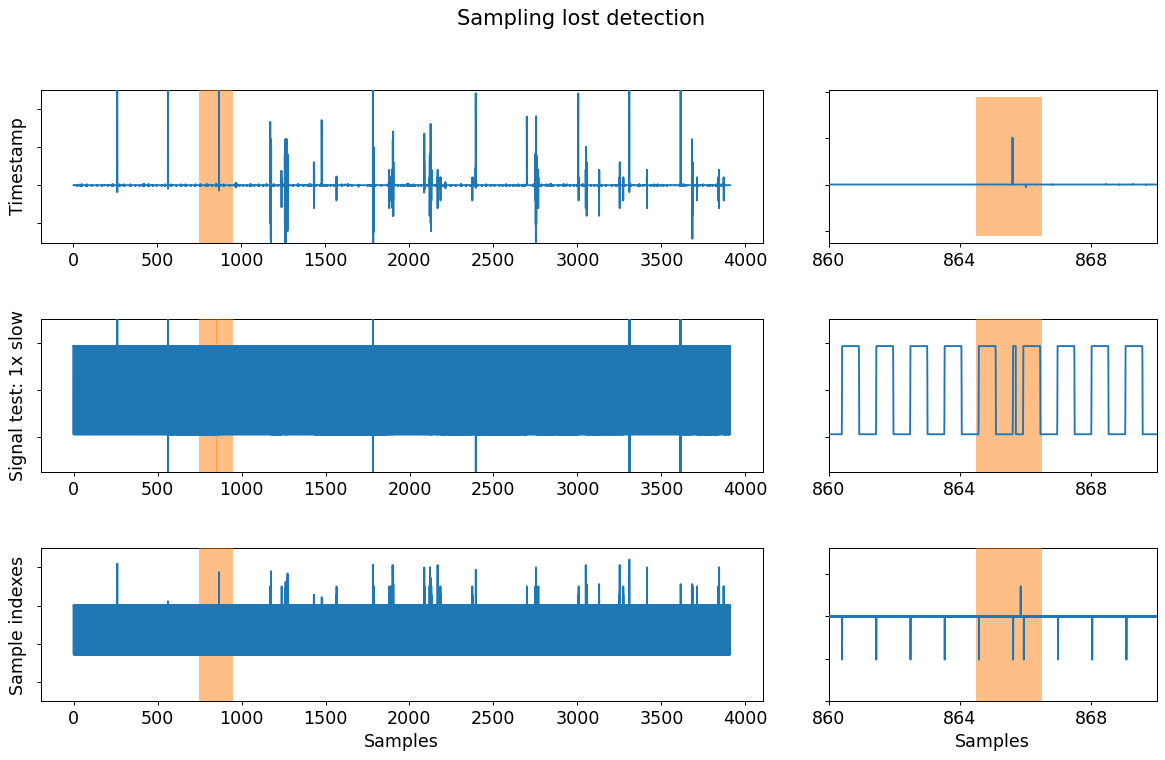
\includegraphics[width=1\textwidth]{Cap3/Figures/sampling_lost_detection.png}
\par\end{centering}
\caption[Sampling lost detection]{The sampling lost can be detected by analysing the timestamp, using a test signal or analysing the sample index.}
\label{fig:sampling_lost_detection}
\end{figure}

For the following analysis, a signal of continuous 64 minutes of acquisition was processed, recorded at 250 SPS, with 100 samples per block size and 16 channels. In Figure \ref{fig:sampling_lost_detection} are compared the three features to detect the samples skips. Any of this methods can be used to locate this points. The selected one is to use the sample indexes, this method has the advantage that can be used with a normal acquisition of EEG, the timestamp also can be used, but is more easy and fast to process the sample indexes. The test signal requires to use the channels for EEG, which makes it less practical.


\begin{figure}
\begin{centering}
% \includesvg[width=0.8\textwidth]{Cap4/Figures/transformer.svg}
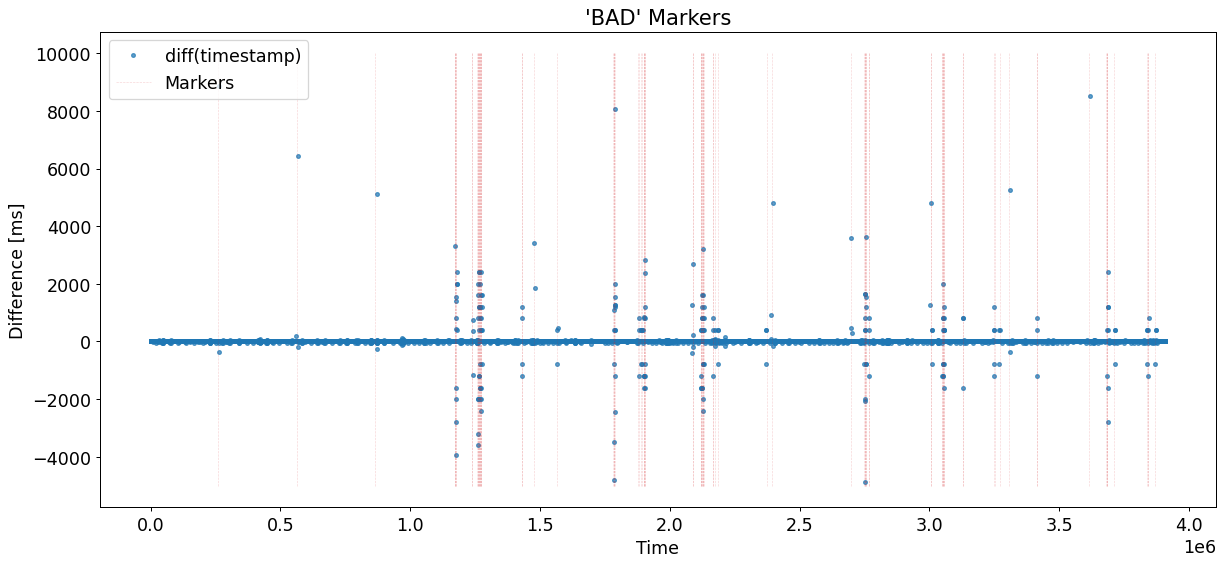
\includegraphics[width=1\textwidth]{Cap3/Figures/bad_markers_autodetection.png}
\par\end{centering}
\caption[Bad markers detection]{The bad markers detection can localize the sampling lost and place markers in that locations.}
\label{fig:bad_markers_autodetection}
\end{figure}

After to perform an algorithm to detect the sampling skips in the signals, this ones are marked as \quot{BAD:sample}. The Figure \ref{fig:bad_markers_autodetection} relates the timestamp with this markers. The \quot{BAD:sample} markers can be used to crop and remove the signal around this ones and to keep with the correctly sampling data. 


\begin{figure}
\begin{centering}
% \includesvg[width=0.8\textwidth]{Cap4/Figures/transformer.svg}
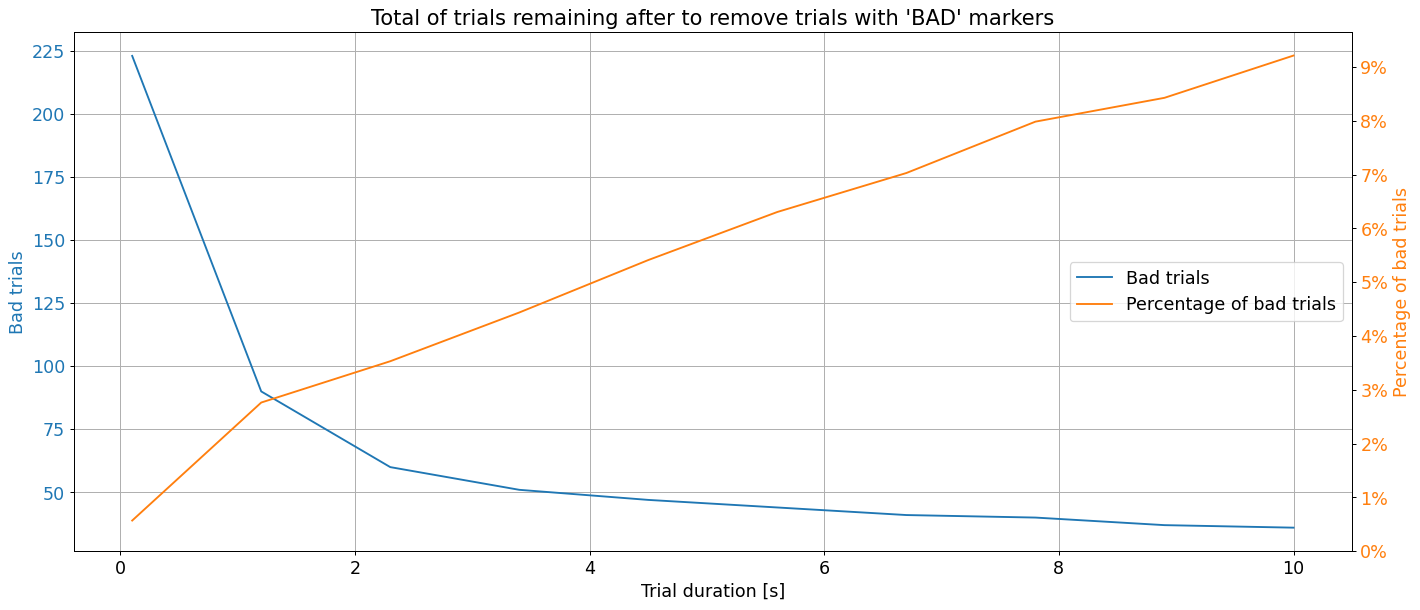
\includegraphics[width=1\textwidth]{Cap3/Figures/trials_remaning.png}
\par\end{centering}
\caption[Trials remaining after to remove trials with 'BAD' markers]{This plot show the trials and the proportion trials remaining after to remove the trials that contain almost one 'BAD' marker for a session of 60 minutes of EEG acquisition, and with a dynamical trial duration between 100 ms to 10000 ms}
\label{fig:trials_remaning}
\end{figure}

In a real experiment is desired a set of trials free of \quot{BAD} markers. The density of this markers can affect a number determined of trials depending of the size of the trial. Figure \ref{fig:trials_remaning} show the results of an experiment of 60 minutes of duration and how many trials must be discarded for each trial duration.

Figure \ref{fig:sampling_rate_analysis} compare the sampling rate around this markers. In the left without remove the skipping points, and in the right after to remove the points identified as bad samples. The right column data are more easy to interpret, the superior plot show the difference of the period in milliseconds, a solid line mark the expected $4 ms$ ($1/250 Hz$), a secondary line $50 ms$ equally distributed above and below. The inferior plot describe the mean of the period for each one of the segments resulting after removing the samples around the \quot{BAD:sample}.


\begin{figure}
\begin{centering}
% \includesvg[width=0.8\textwidth]{Cap4/Figures/transformer.svg}
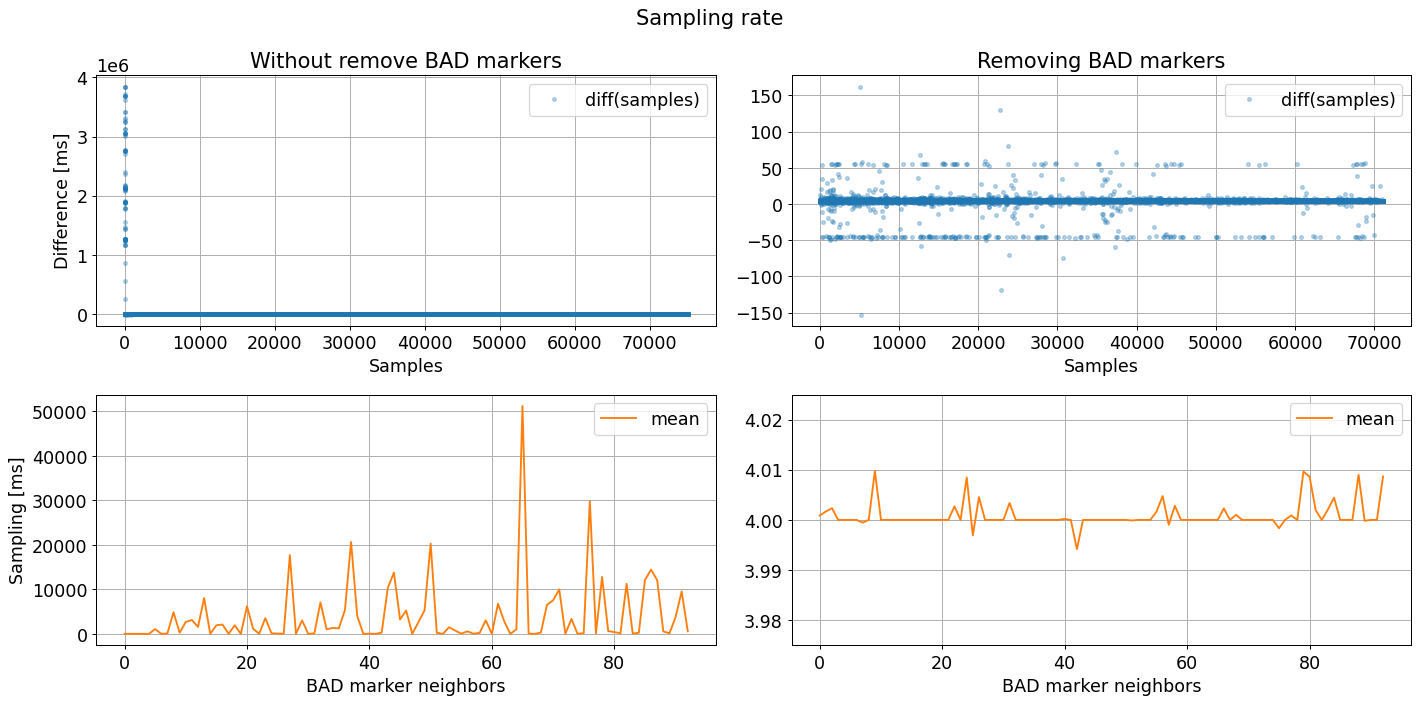
\includegraphics[width=1\textwidth]{Cap3/Figures/sampling_rate_analysis.png}
\par\end{centering}
\caption[Sampling rate analysis after remove bad markers.]{The sampling rate analysis after remove bad markers evidence a data period acquisition close to 4 ms (250 SPS).}
\label{fig:sampling_rate_analysis}
\end{figure}

%======================================================================
\section{Summary and discussion}

The real-time implementation used in this works has been fixed to guarantee the distributions of packages in a time inferior to the package duration itself. Also, the latency measures are expressed in terms of proportion of the acquisition block size, this approach facilitate the comparison with other systems and with the proposed system itself due the different acquisition configuration.

There are two resources used to implement distributed features, the first one is \gls*{RPyC}, this Python module create a remote proxy to access to the drivers module configuration and basic variables. This method use a protocol communication that is too slow to be used to stream EEG in real-time, then Kafka handles this task by implementing a real-time distributed streaming platform. Kafka, also brings other features to generate custom data streams.

The best configuration that integrate, for high sampling rate (1 KSPS), a low and stable latency was the one with fixed transmission block size of 100 samples. This configuration keeps the system stable enough to recover after interruptions and still flexible to implement real-time tasks.

Detect interruptions in the acquired signal is important for the BCI implementations, the performance of the developed systems reside on the quality of the data with which they are fed. Our drivers was designed with the feature to keep and store the data necessary to make this detection and perform automatic purge of bad trials.. 
